\documentclass{article}

% if you need to pass options to natbib, use, e.g.:
% \PassOptionsToPackage{numbers, compress}{natbib}
% before loading nips_2017
%
% to avoid loading the natbib package, add option nonatbib:
% \usepackage[nonatbib]{nips_2017}

\usepackage[final]{nips_2017}

% to compile a camera-ready version, add the [final] option, e.g.:
% \usepackage[final]{nips_2017}

\usepackage[utf8]{inputenc} % allow utf-8 input
\usepackage[T1]{fontenc}    % use 8-bit T1 fonts
\usepackage{hyperref}       % hyperlinks
\usepackage{url}            % simple URL typesetting
\usepackage{booktabs}       % professional-quality tables
\usepackage{amsfonts}       % blackboard math symbols
\usepackage{nicefrac}       % compact symbols for 1/2, etc.
\usepackage{microtype}      % microtypography
\usepackage{graphicx}

\title{Ensemble Learning in Quora Question Intent Matching:
Using Parallel Naive Bayes, Word Embedding, and TF-IDF to Quantify Intent Differences}

% The \author macro works with any number of authors. There are two
% commands used to separate the names and addresses of multiple
% authors: \And and \AND.
%
% Using \And between authors leaves it to LaTeX to determine where to
% break the lines. Using \AND forces a line break at that point. So,
% if LaTeX puts 3 of 4 authors names on the first line, and the last
% on the second line, try using \AND instead of \And before the third
% author name.

\author{
    Nathan M.~Brahmstadt \\
  Department of Electrical and Computer Engineering\\
  Oregon State University\\
  \texttt{brahmstn@oregonstate.edu} \\
  %% examples of more authors
  \And
  Jordan M.~Crane \\
  Department of Electrical and Computer Engineering \\
  Oregon State University \\
  \texttt{cranejo@oregonstate.edu} \\
  %% \AND
  %% Coauthor \\
  %% Affiliation \\
  %% Address \\
  %% \texttt{email} \\
  %% \And
  %% Coauthor \\
  %% Affiliation \\
  %% Address \\
  %% \texttt{email} \\
  %% \And
  %% Coauthor \\
  %% Affiliation \\
  %% Address \\
  %% \texttt{email} \\
}

\begin{document}
% \nipsfinalcopy is no longer used

\maketitle

\begin{abstract}
    Our team set out to solve the problem set forth by the Kaggle Quora Question
    Pairs challenge; that is, to use machine learning and data mining techniques
    to identify Quora questions with similar intent. We aimed to build a model
    that given a pair of questions, could reliably identify whether the
    questions were duplicates or not. Several approaches were explored to
    generate features, and our final classifier leverages all lessons learned
    to minimize our log-loss, which is our primary performance metric. Data was
    filtered strategically to remove noise, fed into four classifiers,
    and combined with a logistic regression model. Through this ensemble
    approach, we achieved 0.4102 log-loss on our training data and 0.3527
    log-loss on our testing data.
\end{abstract}

\section{Approaches explored}

In this section we detail the various approaches that we explored before
settling on our final solution.

\subsection{Pre-processing}

Our pre-processing is primarily carried out by our file parser, which takes the
raw CSV files and pares it down to something that is easier for our main
classifier to work with. It performs several modifications on the data while it
is being parsed.

\subsubsection{Abbreviation expansion}

One technique used by the parser is to look for common abbreviations and
substitute in the expanded version. This is an extremely useful technique, since
it provides the main classifier with more consistency across the data set.

\subsubsection{Stop words}

Another technique that we explored was the removal of stop words in the data.
This approach had both positive and negative ramifications: while it did reduce
the amount of fluff in the data, it also removed some intent-altering words,
such as when, where, and why. Ultimately, it resulted in lower log-loss so we
decided to include it in our final parser.

\subsubsection{Punctuation}

In our initial implementation, the function written to strip punctuation did not
do so properly, which was affecting our results significantly. However, when we
changed it to strip all punctuation, we actually saw an increase in our
log-loss. Further exploration revealed that this was caused by an interesting
feature of the question pairs: in many cases, the last word of the question
holds much greater weight with regard to the question's intent than the
preceding words. By not removing the punctuation, we were unintentionally
setting the last words apart since they were always considered by the classifier
with the question mark included. In order to maintain this unexpected benefit
while still taking advantage of the gains provided by stripping punctuation, we
decided to remove all punctuation, but then duplicate the last word, including
one copy with the question mark and one without. This gave us the lowest
log-loss of all three configurations.

\subsubsection{Spell checking}

At least some of the error in our classifier is the result of one-off
misspellings in the data set. To remedy this, we explored the idea of using a
spell checker to correct the errors in the data. Several factors steered us away
from this approach. Firstly, we couldn't find a spell checking library that was
fast enough to avoid unacceptable slowdown in our parser. Secondly, correcting
all non-dictionary words to dictionary words can incur unintended side effects
by changing intent-altering words that do not appear in common dictionaries,
such as the names of foreign cities or people. Due to these considerations, we
opted not to implement spell checking in our final solution.

\subsection{Classifiers}

\subsubsection{Naive Bayes}

We chose this classifier right off the bat due to our familiarity with it and
how well it lends itself to the problem. However, previous implementations we
had seen were classifying documents independently of one another, not comparing
two separate texts as we are in this problem. In order to overcome this, we
built an ensemble with two Naive Bayes classifiers: one classifier looked at the
words which were common to the two questions, while the other looked at the set
of words which differed. Using the resulting conditional probabilities from
these two bag of words, we could leverage Bayes Theorem and use the resulting
class probabilities as features. We found that these two classifiers in
conjunction were able to make reasonable predictions on a large amount of the
data, since most cases not covered by one were caught by the other. If either
classifier was certain that a question was or was not a duplicate, it overrode
the more uncertain classifier. Smoothing is used in both models to allow for the
words in the test data which are not encountered in training.

\subsubsection{Word embedding}

The other piece of our ensemble's top layer is Google's Word2Vec library
implementing a pre-trained Google News corpus of 3 million 300-dimensional
English word vectors. Word embedding is an interesting approach to natural
language processing which represents words as vectors in a high dimensional
space, such that words with similar usage in context will be placed similarly in
the space. It is famous for its ability to perform analogies, but we tried to
leverage it as a "sentence similarity" measure, with some success. To compute
sentence similarity, we simply use the model to find the average word vector for
both questions, and compute cosine distance between those vectors. This distance
measurement has proven to be a meaningful feature in decreasing our log loss. We
decided to use Google's pre-trained model rather than training our own due to the
relatively small size of our data. There were many words in the training data
that are only seen once, and word embedding performs significantly better after
seeing a word in multiple contexts. We also attempted to quantify sentence
similarity with a variety of other equations, but without success. One idea was
to sum the distance of each word vector to the next word in the question,
providing some insight into word order, context, and word choice. However this
measure failed to increase our accuracy or decrease our loss. This was
definitely the least helpful of the classifiers used in our ensemble, but it
provided a significant reduction to our log-loss, and more insight into certain
question pairs. However, since we are using a pre-trained model word embedding
falls short when it comes to misspellings.

\subsubsection{Total frequency-inverse document frequency}

Term Frequency - Inverse Document Frequency (TF-IDF) weights rarer words with
more importance, similar to Naive Bayes. This method multiplies two frequencies:
the number of times a word appears in a question, and the number of questions
the word appears in. For the term frequency component, we use a binary measure
instead of actual term frequency. This is because term frequency, due to the
short nature of our questions, is almost always 1 anyways because a word is
rarely repeated in questions. In a classifier that deals with longer documents,
term frequency would have more impact. Inverse document frequency is the portion
that we were interested in. We used this metric to represent the word
importance. We computed a "score" to measure question similarity, where positive
points were given if the word was shared, and negative points were given if the
word was not shared. The amount of points given was equal to the TF-IDF, and
this score was calculated by considering all words in both questions.

\subsubsection{Logistic regression}

Logistic regression was the chosen classifier to unify our features for a number
of reasons. It was ideal because it's a relatively simple way to take an
arbitrary number of features, learn weights, and obtain the class probabilities
for the test data. The classifier was used to create a linear decision boundary
for the features that we created from the data. The model is L2 regularized, and
uses a gradient descent solver to converge on a solution.

\subsubsection{Support vector machine}

The final piece of our ensemble was initially a support vector machine to tie
all the other components together. We chose to use an SVM for its simplicity and
ability to group the outputs of the previous classifiers with wide margin. It
also came with the added benefit that the results are easily plotted. Visualizing the
data benefited us because we could obtain a better intuition about our
classifier's performance, and more easily share our results with others.
However, while methods exist to calculate distances of samples to the SVM
decision line in order to extract probabilities, ultimately, logistic regression
became the best and easiest method to obtain our final results from our
features.

\subsubsection{Convolutional neural network}

We also explored using a convolutional neural network to form our decision
boundary but found it to be overly complex for the task. Additionally, we
worried that a more complex model would over fit, and were unsure of our ability
to combat this in an ensemble.

\subsubsection{Long short-term memory network}

The most advanced classifier that we explored was a long short-term memory
network (LSTM). This is a type of recurrent neural network that excels at
natural language processing due to its ability to remember information for long
periods of time through the recurrent behavior of the network. This memory gives
it the ability to interpret context much more effectively even when compared to
other kinds of recurrent neural networks. We used the LSTM layer provided in
Keras to test various configurations, but ultimately decided not to use the
classifier for several reasons. Firstly, while LSTMs do excel at natural
language processing, they are typically used with a single text input, and in
order to use one with the two-question inputs from our problem required more
advanced usage of Keras input layers to concatenate the inputs. Additionally,
our team had no prior familiarity with Keras even in the context of simple
problems and networks, and jumping straight into a fairly complex use case
proved to be daunting. Ultimately, between the difficulty in representing the
data and our unfamiliarity with the framework, we decided to opt for something
simpler to allow us to perform more intelligent optimization on a model we knew
more intimately.

\section{Results}

In this section we explore the results of our explorations, how we improved our
model over time, and the limitations of our chosen model.

\subsection{Exploration results}

Our initial approach of using two Naive Bayes models was only slightly above
50\% accuracy on training data. This was improved drastically with
pre-processing, which was able to bring that accuracy to over 70\%. Our testing
log-loss was 0.435 with this model. At this point, we searched for another
feature to add, which is when we started experimenting with word embedding. The
only sentence similarity measure that improved our performance was comparing the
average word vector values of the question pair, which brought up our testing
accuracy to 77\% and our testing log-loss to 0.41. In our search for additional
features, we also found the TF-IDF formula, which perfectly summed up our
intuition about word rarity’s effect on the intent. After implementing TF-IDF,
we increased our training accuracy by 1\%. Exploring variations of this
equation, including using binary frequency instead of actual, and smoothing
document frequency (Similar to Naive Bayes smoothing), netting a few more
percentage points. Overall, TF-IDF brought us to 0.39 log-loss on the testing
data. At this point, we went back to the pre-processing options to explore its
effect on our variety of features. Keeping question marks, removing stop words,
and a few other ideas mentioned above all yielded slight improvements in
log-loss. The sum of all of these changes brought the log-loss to 0.3527 on the
testing data.

\begin{figure}[h]
    \centering
    \mbox{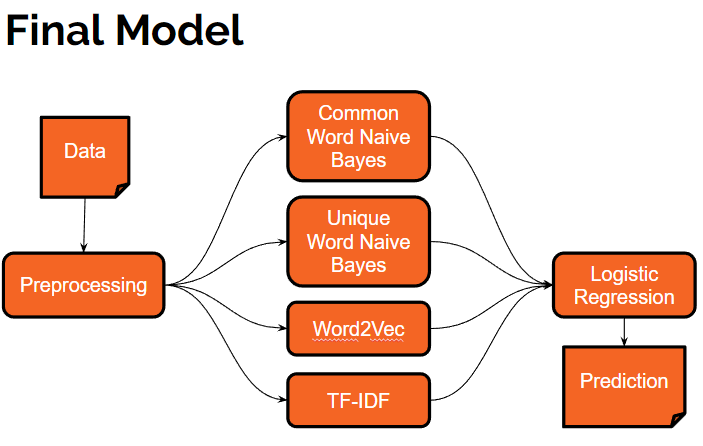
\includegraphics[width=100mm]{block_diagram.png}}
    \caption{Block diagram of final ensemble}
\end{figure}

\subsection{Possible improvements}
There are several limitations to our model that we think could be addressed to
yield even better results in the future.

\subsubsection{Word order} First, none of features take word order into
consideration (except the last word doubling that we do in pre-processing). The
last-word doubling alone brought our log-loss from 0.37 to 0.35. Perhaps there’s
other word order features like common word pairs (“new york”, “harry potter”,
etc) or the first word of each question that could improve our classifier. We
did attempt this in several ways like measuring word vector distances, and
giving TF-IDF pairs of words, but these yielded either no net improvement or
worse overall performance.

\subsubsection{Multiple pre-proccessed training data sets}

Our exploration can attest to the power of pre-processing for this problem, with
dramatic improvements attained with simple steps like removing punctuation.
However, we also see value in keeping things like stop words, as removing them
can make two different intent questions identical in some cases. We attempted
this by creating several classifiers trained on different parsed data, and
feeding all of the resulting features into a single logistic regression
function, but it dramatically reduced our performance. Perhaps with a different
structure, like a neural network, this could increase performance.

\subsubsection{Word-embedding model choice}

Instead of using a model trained from Google News, other sources might be more
meaningful. News articles probably don’t consist of too much slang or spelling
errors, therefore the model has no representation for those things, which are
numerous in the Quora Data. We tried to train the model on the Quora data, but
that was less meaningful than the Google model. Perhaps some combination of
them, or a model trained from Reddit or Facebook, where more casual
conversations occur, would benefit our results.

\subsubsection{Word relationships and synonyms}

Word relation is a problem that we attempted to solve with word-embedding, but
we still feel that could be improved. There are many questions with the same
intent that do not share the same phrasing, but have the same intent. Words like
“code” and “programming” are related, but our classifier doesn’t often see a
strong enough relationship between them to realize that they represent similar
intent. Perhaps more weight could be put on the word embedding portion of our
classifier to address this, or find another way to represent synonyms.

\section{Conclusion} \label{headings} Our goal was to create meaningful
classifiers exploring the concept of "differing and shared words" as
identifiers of intent between two questions. The resulting ensemble approach
unified three meaningful classifiers that we had discovered, and obtained a
0.35274 log-loss on the test data. This score is by no means ground-breaking,
but we are satisfied by the result anyways. Our approach was able to perform
above average in the competition, and we feel that the success it had, based on
its relatively simple algorithm, exceeded our expectations.

\section*{Appendix: contribution levels}

\subsection*{Nathan - 50\%}
Performed exploration relating to the TF-IDF, Word Embedding, and Naive Bayes classifiers.

\subsection*{Jordan - 50\%}
Performed exploration relating to pre-processing, Keras, and LTSM networks.

\end{document}
